\documentclass{beamer}

\usepackage{textcomp}
\usepackage{xcolor}
\usepackage{listings}
% \usepackage{matlab-prettifier}
\usepackage[T1]{fontenc}
\usepackage{multimedia}
\usepackage{hyperref}

\usepackage{caption}
\captionsetup{justification=raggedright,singlelinecheck=false}

\usetheme{Boadilla}

\makeatletter
\def\blfootnote{\gdef\@thefnmark{}\@footnotetext}
\makeatother
\urlstyle{sf}

\title{Crabsort}
\subtitle{Spike-sorting for small circuit networks}
\author{Alec Hoyland & Cosmo Guerini}
\institute[CSN]{Center for Systems Neuroscience}

\begin{document}

%% title page

\begin{frame}
  \titlepage
\end{frame}


\section{Introduction}

% introduce the problem
% What is spike sorting? Why does it matter?
% How can machine learning help?

\begin{frame}
  \frametitle{Spike-sorting primer}

  Spike-sorting is the process of mapping action potentials to the originating cell.

  \begin{columns}
    \column{0.5\textwidth}

    \begin{figure}
      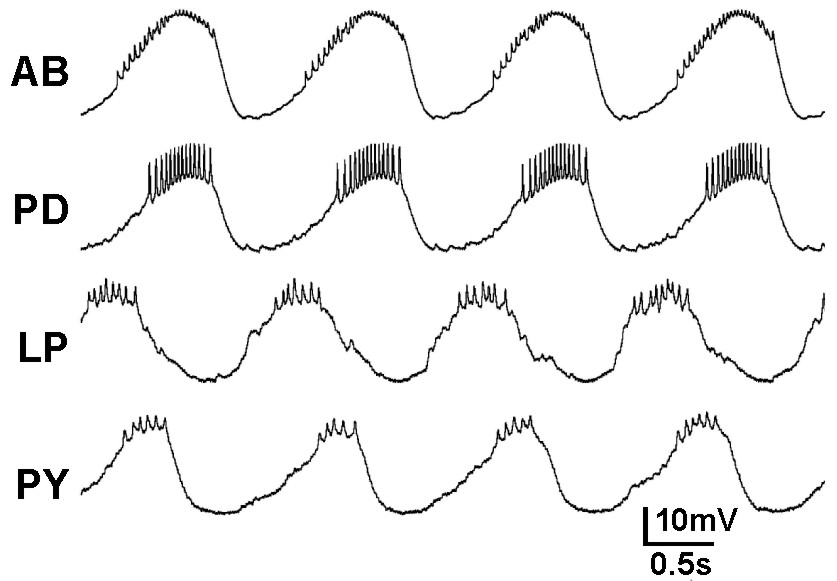
\includegraphics[width=\textwidth]{gfx/pyloric.jpeg}
      \centering
      \caption{Intracellular recordings of pyloric cells.}
      \label{fig:intracellular}
    \end{figure}

    \column{0.5\textwidth}

    \begin{figure}
      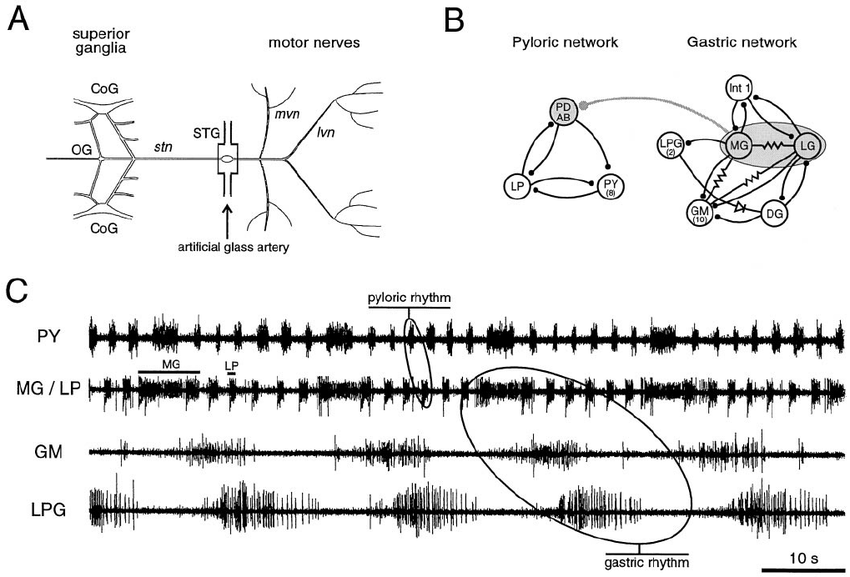
\includegraphics[width=\textwidth]{gfx/STG-rhythms.png}
      \centering
      \caption{\textbf{A} circuit diagram of nerves; \textbf{B} connectivity diagram, circles are cells, synapses are lines and dots; \textbf{C} extracellular recording of motor nerves.}
      \label{fig:extracellular}
    \end{figure}

  \end{columns}

\end{frame}

% introduce how to sort spikes
% Small circuits vs. large circuits.
% Why large circuit solutions don't work for small circuits.

\begin{frame}
  \frametitle{How to sort spikes}

  \begin{enumerate}
    \item Identify spikes from membrane potential waveform (easy)
    \item Sort spikes using some magic algorithm (hard)
  \end{enumerate}

  \medskip

  \begin{columns}
    \column{0.5\textwidth}

    For large networks, spike sorting means:

    \begin{enumerate}
      \item Methods: PCA, SVD, stochastic k-means matching of correllograms
      \item Data: 100s of channels but without a ground truth
    \end{enumerate}

    \medskip

    For small networks, spike sorting means:

    \begin{enumerate}
      \item Methods: dimensionality reduction, machine learning
      \item Data: few channels with known activity
    \end{enumerate}

    \column{0.5\textwidth}

    \begin{figure}
      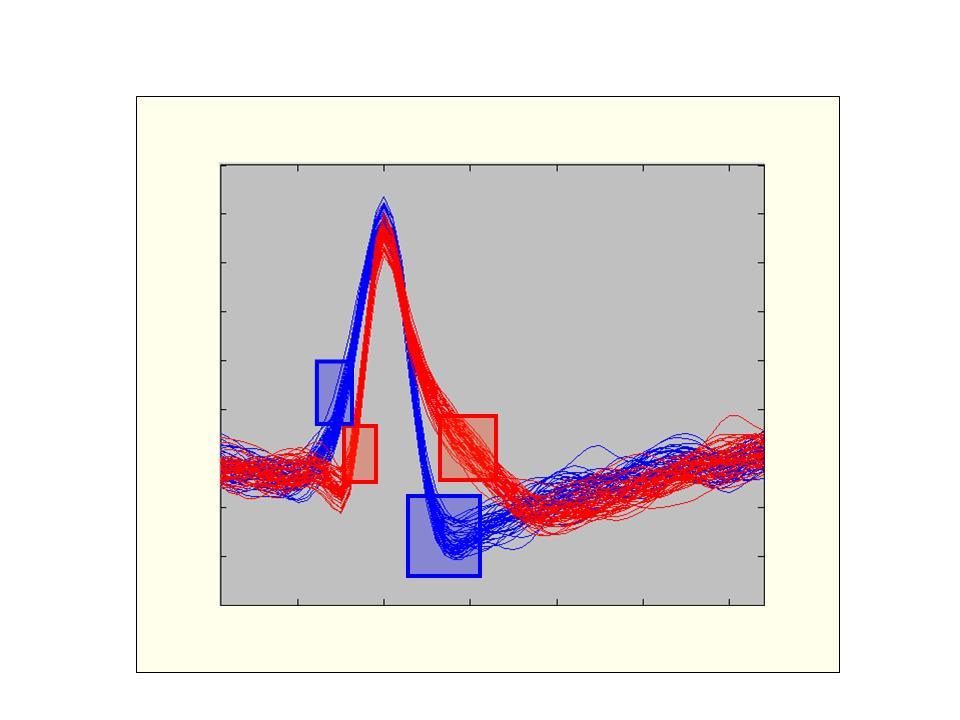
\includegraphics[width=\textwidth]{gfx/spike-sorting.jpeg}
      \centering
      \caption{Spike-sorting using PCA and window filtering by spike-waveform analysis (R. Quian Quiroga).}
      \label{fig:spikesorting}
    \end{figure}

  \end{columns}

\end{frame}

% introduce crabsort
% what are the steps? dimensionality reduction, training the NN, using the NN

\section{Crabsort}

\begin{frame}
  \frametitle{Crabsort}
\end{frame}

% dimensionality reduction
% why is it important?
% how does crabsort do it?
% what are the different kinds?

\begin{frame}
  \frametitle{Dimensionality Reduction}

  Dimensionality reduction is the process of taking high-dimensional data
  and representing it in a lower dimensional space.

  Crabsort allows the user to:

  \begin{enumerate}
    \item Dimensionally reduce the data to a 2-dimensional manifold
    \item Interactively label the data
  \end{enumerate}

  \begin{figure}
    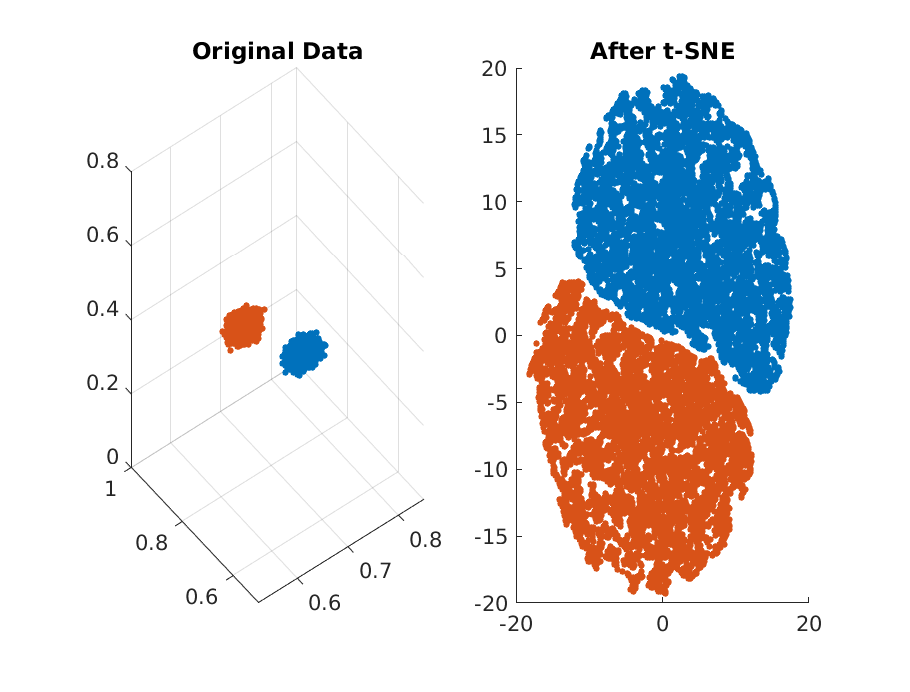
\includegraphics[width=0.5\textwidth]{gfx/t-SNE-example.eps}
    \centering
    \caption{Using the t-SNE algorithm to reduce a 3-dimensional dataset to a 2-dimensional dataset.}
    \label{fig:dimredexample}
  \end{figure}


\end{frame}

% t-SNE and FIt-SNE

\begin{frame}[t]
  \frametitle{t-distributed stochastic neighborhood embedding}

  \begin{columns}
    \column{.5\linewidth}

    \begin{enumerate}
      \item Choose nearest neighbors for $x_i$ via a multi-dimensional Gaussian probability distribution centered at $x_i$.
      \item Compute t-distributed similarity measure in low-dimensional space.
      \item Minimize the Kullback-Leibler divergence between the high-dimensional distribution and the low-dimensional distribution.
    \end{enumerate}


    \column{.5\linewidth}

    With FFT-interpolation

    \begin{enumerate}
      \item Computing objective function requires a convolution.
       So, interpolated equispaced grid, and compute convolution
       in Fourier space using FFT.
       \item Use approximate nearest neighbors (ANNOY) to multithread kNN task.
       \item 15-30x faster at $\mathcal{O}(n \log n)$.
    \end{enumerate}

  \end{columns}

\end{frame}

% UMAP

\begin{frame}
  \frametitle{Uniform manifold approximation and projection}

  \begin{columns}
    \column{0.5\textwidth}

    \begin{enumerate}
      \item k-nearest neighbors leads to a weighted graph
      which defines a manifold
      \item Spectral clustering on the Laplacian matrix
      \item Minimization of fuzzy simplicial set cross entropy optimizes embedding.
    \end{enumerate}

    \column{0.5\textwidth}

    \begin{figure}
      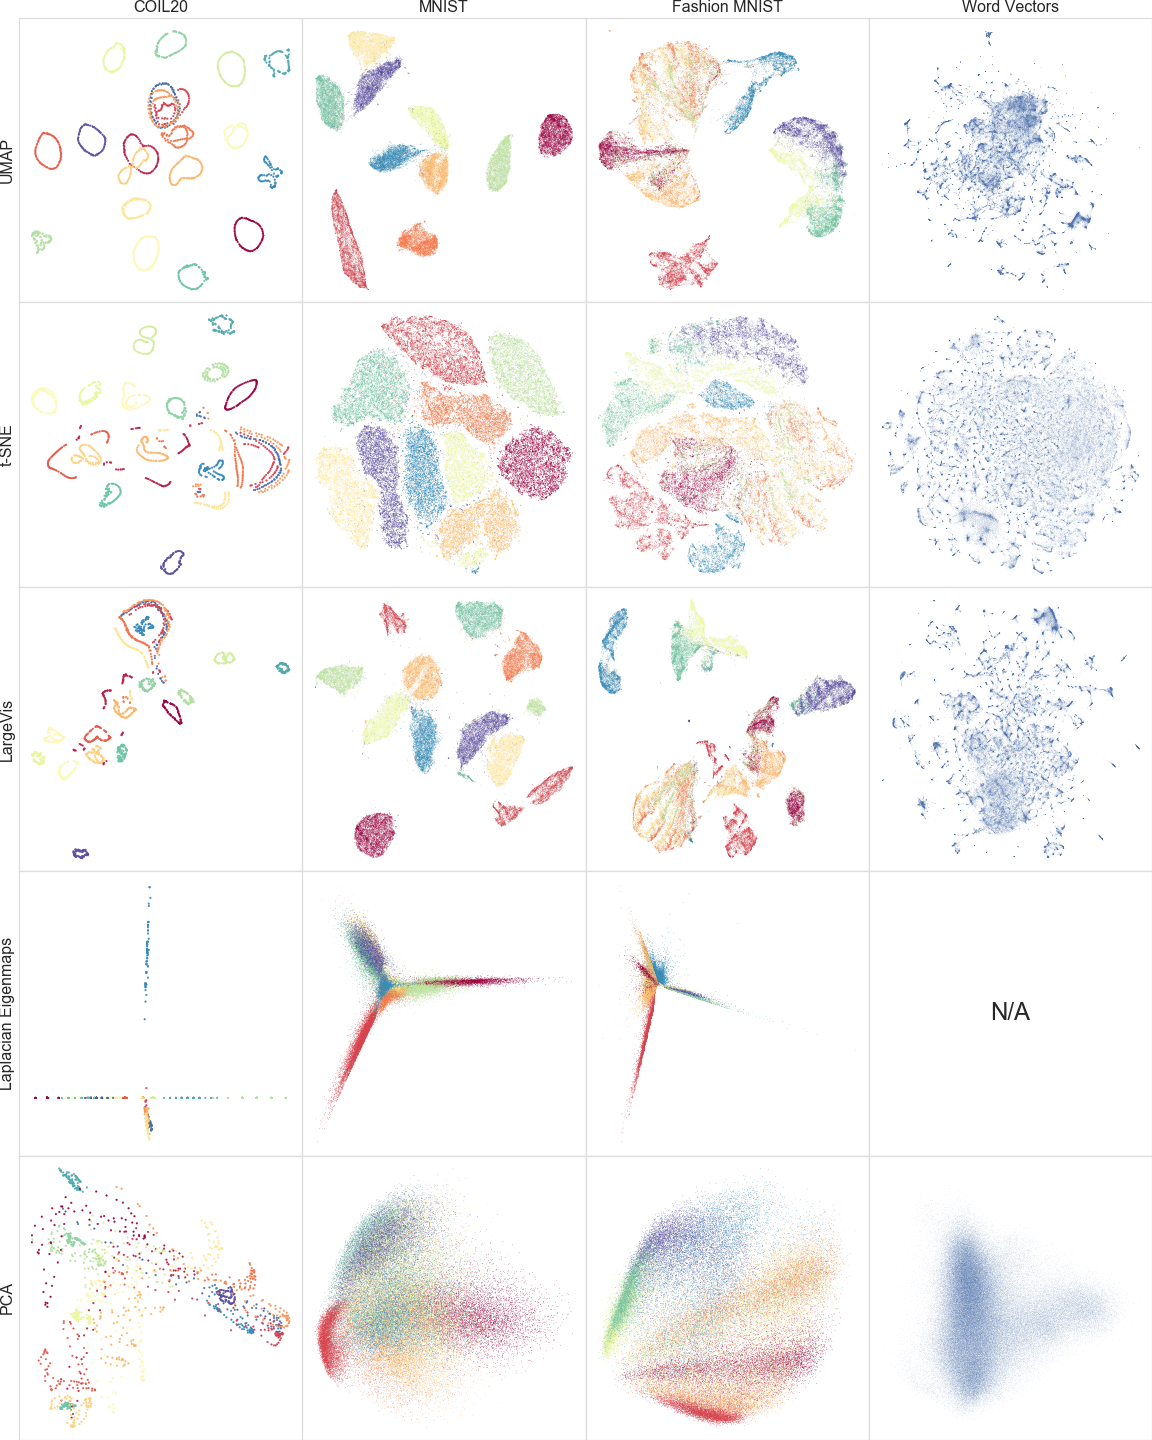
\includegraphics[width=0.75\textwidth]{gfx/umap.png}
      \centering
      \caption{Comparison of UMAP, t-SNE and other dimensional reduction techniques.}
      \label{fig:dimredcompare}
    \end{figure}

  \end{columns}

\end{frame}

\end{document}
